% !TEX root = C:\Users\Jan\Documents\dev\Risk-Measurement-Framework\masterthesis_tex\masterthesis_main.tex
\section{Evaluation}
\label{sec:evaluation}

A common example to show backdoor attacks is traffic sign detection (\cite{DBLP:journals/corr/abs-2102-10369}, \cite{DBLP:journals/corr/abs-1708-06733}, \cite{DBLP:conf/codaspy/NudingM20}, \cite{DBLP:journals/tdsc/LiXZZZ21}). That makes it easier to find datasets and already finished ML models to make a case study. In the following subsections the focus lies on the case study which concept and its implementation is evaluated here. In addition, this section describes real-world examples for which the RMF could be used.

\subsection{Evaluation of the ISO 27004 standard in context to the RMF}

After mapping the ISO 27004 to the RMF one result is that this standard should be mapped to a framework if the process stands in relation to a organization and an implemented ISMS.

\subsection{Case Study: Developing a SVM for traffic sign detection}

For the case study scikit-learn \cite{scikit-learn} and for preparation of the dataset in Python OpenCV2 have different function to load and resize images \cite{opencv_library}. In their work, Stallkamp et al. \cite{DBLP:conf/ijcnn/StallkampSSI11} built a mulit-category classification dataset. The mulit-category classification dataset contains german traffic signs for image classification. That mulit-category classification dataset uses the german traffic signs from a approx. 10 hours daytime video from different roads.
This case study is an example to show the functions and results of the RMF. After showing this case study there will be explain and discuss realistic case studies where backdoor attacks could have a more realistic impact for scores of ML models.

\subsection{Structure of the ML model for the case study}

The original dataset from Stallkamp et al. \cite{DBLP:conf/ijcnn/StallkampSSI11} is splitted between a training and testing folder. The training folder separate 43 signs into subfolders. This subfolders make it easy to use specific traffic signs which decrease the training time. The information of the folders are written in an eponymous csv-file that are not needed further in this case study. In Figure \ref{fig:traffic_signs} the shown traffic signs can be used for training the SVM and are all labeled in the data preprocessing like the subfolder name 0 - 42.

\begin{figure}[h!]
  \centering
  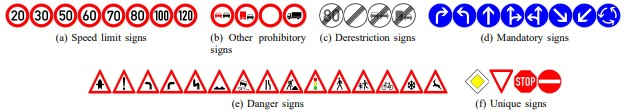
\includegraphics[width=12cm]{pictures/traffic_signs.jpg}
  \caption{Labeled traffic signs adapted from \cite{DBLP:conf/ijcnn/StallkampSSI11}}
  \label{fig:traffic_signs}
\end{figure}

\begin{figure}[h!]
  \centering
  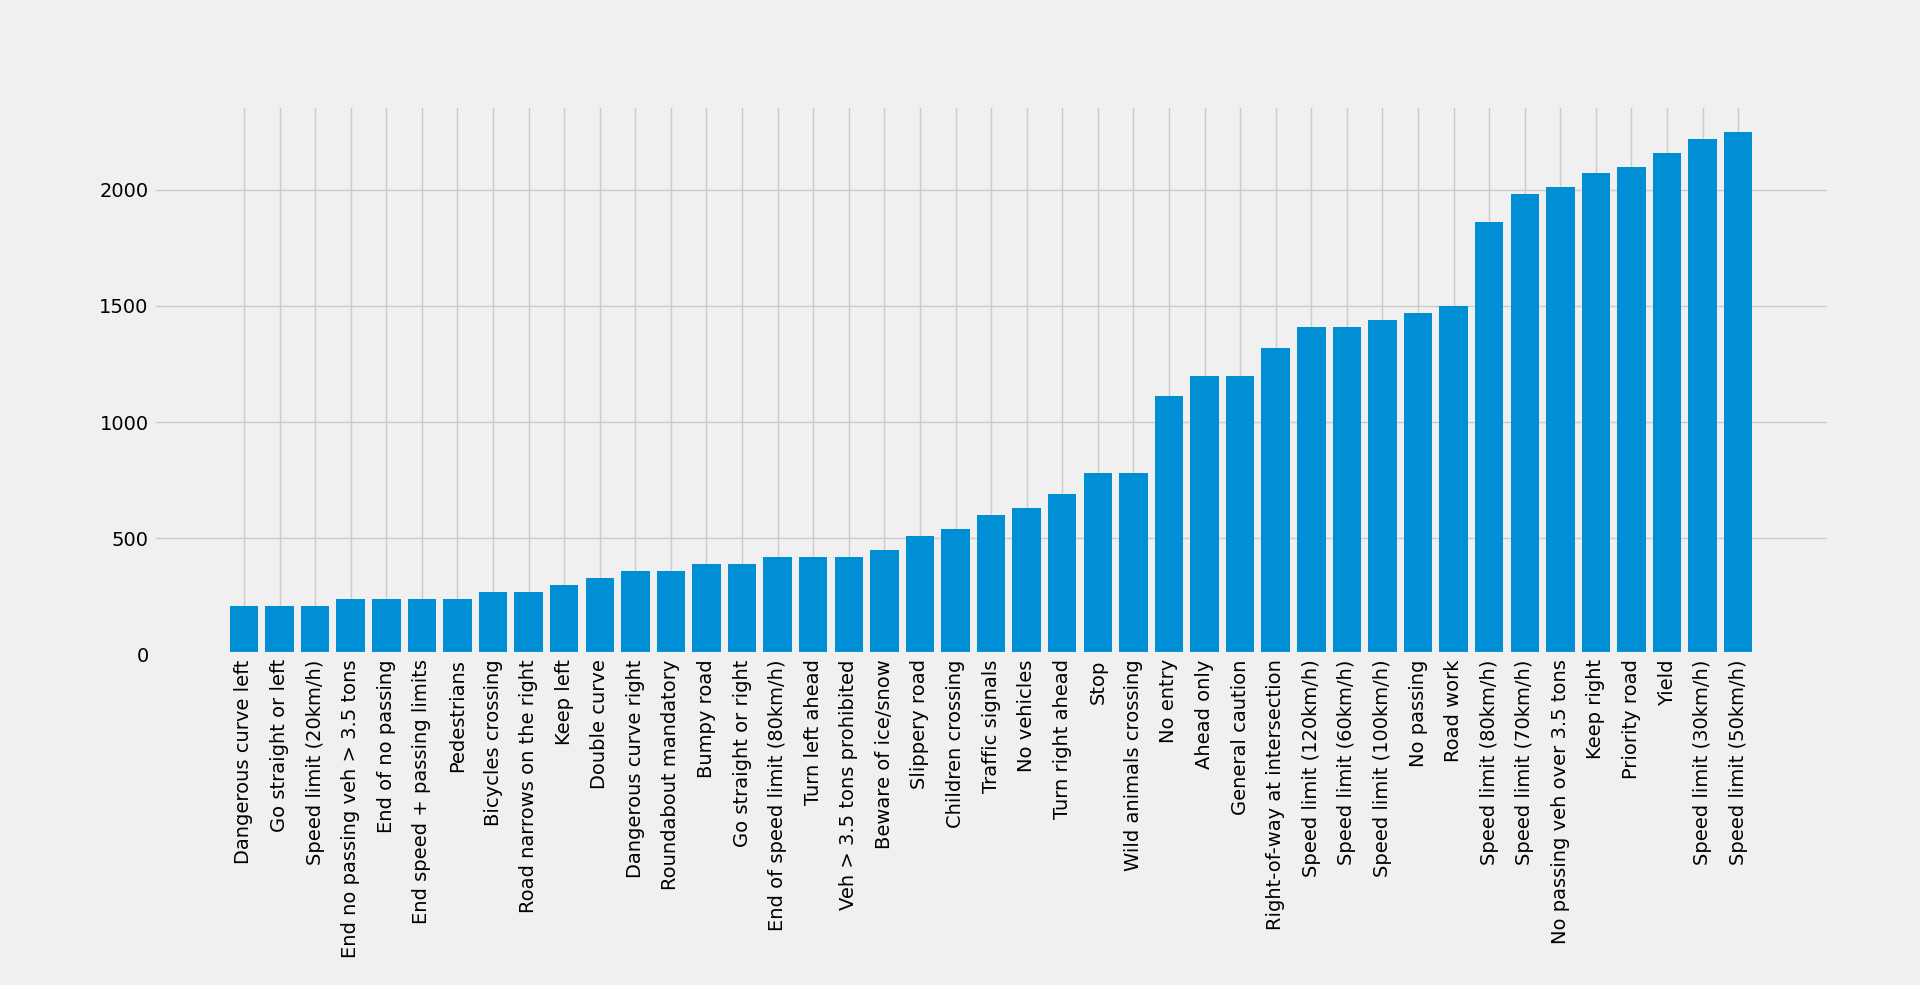
\includegraphics[width=15cm]{pictures/num_of_images.png}
  \caption{Number of images per labels}
  \label{fig:num_of_images}
\end{figure}

All signs are resized to 30x30 pixel to optimize the performance of the NN. The training sets are also scaled with Keras and TensorFlow to execute the attacks successfully. The training data and test data load from two different folders. All functions, the arguments and a description of them can be found in appendix \ref{sec:case_study_functions}. Figure \ref{fig:nn} shows the NN architecture.

\begin{figure}[h!]
  \centering
  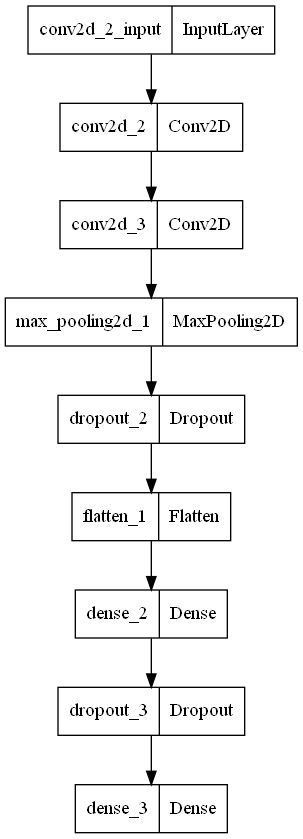
\includegraphics[width=5cm]{pictures/nn.png}
  \caption{Generated NN architecture image from Keras}
  \label{fig:nn}
\end{figure}

The computer to execute the ML model have resources such as, AMD Ryzen \cite{DBLP:conf/hotchips/AroraBW20} 7 5800X 8-Core Processor with 3.80 GHz, 16 GB of RAM, and a NVIDIA GeForce RTX \cite{DBLP:journals/pcs/SanzharovFG20} 3060 Ti. These resources can be used for the risk indicator computational resources to measure the original and attacked ML model.

\subsubsection*{Expected results of the case study}

\subsection{Differences between manipulated and original dataset}

The Python plots from the case study show in this subsection examples images to show the differences between the original and manipulated dataset.

\subsection{Results from the risk measurement based on the risk indicators}

\subsubsection*{Risk indicators to measure the attacker's effort}
\textbf{Attacker's goal} \\
\textbf{Attacker's knowledge} \\
\textbf{Computational resources} The computational resources that are measured are the CPU, GPU, and RAM. The RAM measurement starts at the beginning of the implemented ML model and shows after finishing the training and testing time of the ML model how much RAM resources the ML model used. When the ML model has no attacks implemented, the ML model needs \%

\subsubsection*{Risk indicators to measure the extent of damage}
\textbf{Attack time} All backdoor attacks are executing during training time. \\
\textbf{Positiv and negative label} \\
\textbf{Accuracy} The accuracy is a risk indicator should be decreased as much as possible if an ML model is attacked with a backdoor attack. The original ML model has an accuracy of $96\%$ \\
\textbf{Attack specificity} The \textit{PoisoningAttackBackdoor} is a untargeted attack, \textit{PoisoningAttackCleanLabelBackdoor} is a targeted attack, and the \textit{HiddenTriggerBackdoor} is a targeted attack.

\subsection{Poisoning and backdoor attacks in real applications}

Beside the exemplary application from the case study, the scientific papers in this subsection show real applications where the RMF can then help in a more real environment. An example for real-world poisoning attacks against ML models is Microsoft's chatbot Tay. This chatbot learned racist and offensive language from Twitter users \cite{DBLP:conf/iciot/BaracaldoCLSZ18}, \cite{DBLP:conf/ccs/BaracaldoCLS17}. Microsoft removed the bot after 16 hours because the bot produced offensive tweets.
